%%%%%%%%%%%%%%%%%%%%%%%%%%%%%%%%%%%%%%%%%%%%%%%%%%%%%%%%%%%%%%%%%%%%%%%%%%%
%% This file is part of the book
%%
%% Algorithmic Graph Theory
%% http://code.google.com/p/graph-theory-algorithms-book/
%%
%% Copyright (C) 2009, 2010, 2011 Minh Van Nguyen <nguyenminh2@gmail.com>
%%
%% See the file COPYING for copying conditions.
%%%%%%%%%%%%%%%%%%%%%%%%%%%%%%%%%%%%%%%%%%%%%%%%%%%%%%%%%%%%%%%%%%%%%%%%%%%

\subfigure[Original graph.]{
\label{fig:separating_set:original_graph}
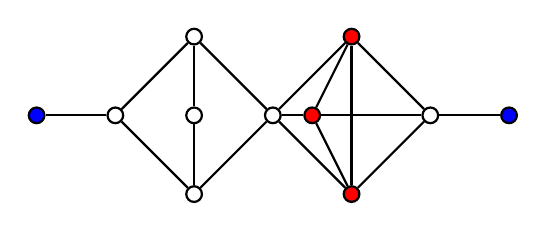
\begin{tikzpicture}
[nodeDecorate/.style={shape=circle,inner sep=2pt,draw,thick},%
  lineDecorate/.style={-,thick},scale=1]
%% nodes or vertices
\foreach \nodename/\x/\y in {
  0/0/0, 2/2/0, 6/-1/1, 7/-1/0, 8/-1/-1, 9/-2/0}
{
  \node (\nodename) at (\x,\y) [nodeDecorate] {};
}
\foreach \nodename/\x/\y/\fillcolor in {
  1/0.5/0/red, 3/3/0/blue, 4/1/-1/red, 5/1/1/red, 10/-3/0/blue}
{
  \node (\nodename) at (\x,\y) [nodeDecorate,fill=\fillcolor] {};
}
%% edges or lines
\path
\foreach \startnode/\endnode in {
  0/1, 0/4, 0/5, 0/6, 0/8, 1/2, 1/4, 1/5, 2/3, 2/4, 2/5, 4/5, 6/7,
  6/9, 7/8, 8/9, 9/10}
{
  (\startnode) edge[lineDecorate] node {} (\endnode)
};
\end{tikzpicture}
}
%%
%%
\qquad
\subfigure[Vertex separated.]{
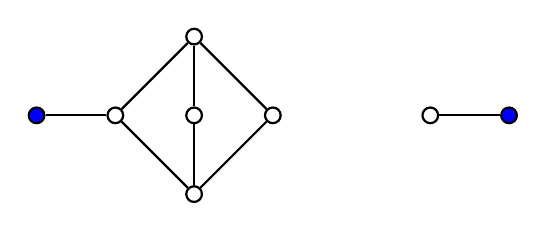
\begin{tikzpicture}
[nodeDecorate/.style={shape=circle,inner sep=2pt,draw,thick},%
  lineDecorate/.style={-,thick},scale=1]
%% nodes or vertices
\foreach \nodename/\x/\y in {
  0/0/0, 2/2/0, 6/-1/1, 7/-1/0, 8/-1/-1, 9/-2/0}
{
  \node (\nodename) at (\x,\y) [nodeDecorate] {};
}
\node (3) at (3,0) [nodeDecorate,fill=blue] {};
\node (10) at (-3,0) [nodeDecorate,fill=blue] {};
%% edges or lines
\path
\foreach \startnode/\endnode in {
  0/6, 0/8, 2/3, 6/7, 6/9, 7/8, 8/9, 9/10}
{
  (\startnode) edge[lineDecorate] node {} (\endnode)
};
\end{tikzpicture}
}
%%
%%
\subfigure[Original graph.]{
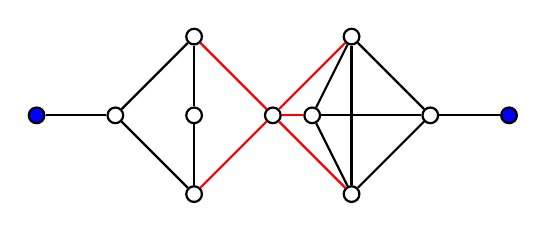
\begin{tikzpicture}
[nodeDecorate/.style={shape=circle,inner sep=2pt,draw,thick},%
  lineDecorate/.style={-,thick},scale=1]
%% nodes or vertices
\foreach \nodename/\x/\y in {
  0/0/0, 1/0.5/0, 2/2/0, 4/1/-1, 5/1/1, 6/-1/1, 7/-1/0, 8/-1/-1, 9/-2/0}
{
  \node (\nodename) at (\x,\y) [nodeDecorate] {};
}
\node (3) at (3,0) [nodeDecorate,fill=blue] {};
\node (10) at (-3,0) [nodeDecorate,fill=blue] {};
%% edges or lines
\path
\foreach \startnode/\endnode in {
  1/2, 1/4, 1/5, 2/3, 2/4, 2/5, 4/5, 6/7, 6/9, 7/8, 8/9, 9/10}
{
  (\startnode) edge[lineDecorate] node {} (\endnode)
}
\foreach \startnode/\endnode/\edgecolor in { 0/1, 0/4, 0/5, 0/6, 0/8}
{
  (\startnode) edge[lineDecorate,color=red] node {} (\endnode)
};
\end{tikzpicture}
}
%%
%%
\qquad
\subfigure[Edge separated.]{
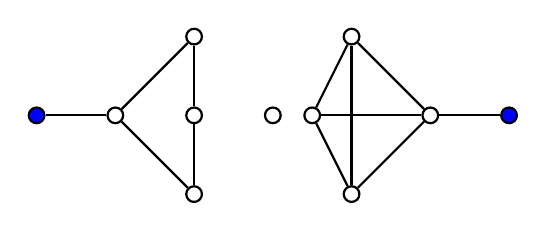
\begin{tikzpicture}
[nodeDecorate/.style={shape=circle,inner sep=2pt,draw,thick},%
  lineDecorate/.style={-,thick},scale=1]
%% nodes or vertices
\foreach \nodename/\x/\y in {
  0/0/0, 1/0.5/0, 2/2/0, 4/1/-1, 5/1/1, 6/-1/1, 7/-1/0, 8/-1/-1, 9/-2/0}
{
  \node (\nodename) at (\x,\y) [nodeDecorate] {};
}
\node (3) at (3,0) [nodeDecorate,fill=blue] {};
\node (10) at (-3,0) [nodeDecorate,fill=blue] {};
%% edges or lines
\path
\foreach \startnode/\endnode in {
  1/2, 1/4, 1/5, 2/3, 2/4, 2/5, 4/5, 6/7, 6/9, 7/8, 8/9, 9/10}
{
  (\startnode) edge[lineDecorate] node {} (\endnode)
};
\end{tikzpicture}
}
